\documentclass[12pt,a4paper]{report}

% Import des packages 
\usepackage[french]{babel}
\usepackage[utf8x]{inputenc}
\usepackage[T1]{fontenc}
\usepackage[dvipsnames]{xcolor}
\usepackage{titlesec}
\usepackage{blindtext}
\usepackage{geometry}
\usepackage{graphicx}
\usepackage[font=small,labelfont=bf]{caption}

%Define the listing package
\usepackage{listings} %code highlighter
\usepackage{color} %use color
\definecolor{mygreen}{rgb}{0.2,0.7,0.1}
\definecolor{mygray}{rgb}{0.5,0.5,0.5}
\definecolor{mymauve}{rgb}{0.58,0,0.82}

%Customize a bit the look
\lstset{
	backgroundcolor=\color{white}, % choose the background color; you must add \usepackage{color} or \usepackage{xcolor}
	basicstyle=\footnotesize, % the size of the fonts that are used for the code
	breakatwhitespace=false, % sets if automatic breaks should only happen at whitespace
	breaklines=true, % sets automatic line breaking
	captionpos=b, % sets the caption-position to bottom
	commentstyle=\color{mygreen}, % comment style
	deletekeywords={...}, % if you want to delete keywords from the given language
	escapeinside={\%*}{*)}, % if you want to add LaTeX within your code
	extendedchars=true, % lets you use non-ASCII characters; for 8-bits encodings only, does not work with UTF-8
	frame=single, % adds a frame around the code
	keepspaces=true, % keeps spaces in text, useful for keeping indentation of code (possibly needs columns=flexible)
	keywordstyle=\color{blue}, % keyword style
	% language=Octave, % the language of the code
	morekeywords={*,...}, % if you want to add more keywords to the set
	numbers=left, % where to put the line-numbers; possible values are (none, left, right)
	numbersep=5pt, % how far the line-numbers are from the code
	numberstyle=\tiny\color{mygray}, % the style that is used for the line-numbers
	rulecolor=\color{black}, % if not set, the frame-color may be changed on line-breaks within not-black text (e.g. comments (green here))
	showspaces=false, % show spaces everywhere adding particular underscores; it overrides 'showstringspaces'
	showstringspaces=false, % underline spaces within strings only
	showtabs=false, % show tabs within strings adding particular underscores
	stepnumber=1, % the step between two line-numbers. If it's 1, each line will be numbered
	stringstyle=\color{mymauve}, % string literal style
	tabsize=2, % sets default tabsize to 2 spaces
	title=\lstname % show the filename of files included with \lstinputlisting; also try caption instead of title	
}

%END of listing package%

% On définit des couleurs perso
\definecolor{darkgray}{rgb}{.4,.4,.4}
\definecolor{purple}{rgb}{0.65, 0.67, 0.69}

%definition d'un modèle d'un style pour JS
\lstdefinelanguage{JavaScript}{
	keywords={typeof, new, true, false, catch, function, return, null, catch, switch, var, if, in, while, do, else, case, break},
	keywordstyle=\color{blue}\bfseries,
	ndkeywords={class, export, boolean, throw, implements, import, this},
	ndkeywordstyle=\color{darkgray}\bfseries,
	identifierstyle=\color{black},
	sensitive=false,
	comment=[l]{//},
	morecomment=[s]{/*}{*/},
	commentstyle=\color{mygreen}\ttfamily,
	stringstyle=\color{red}\ttfamily,
	morestring=[b]',
	morestring=[b]"
}

\lstset{
	language=JavaScript,
	extendedchars=true,
	basicstyle=\footnotesize\ttfamily,
	showstringspaces=false,
	showspaces=false,
	numbers=left,
	numberstyle=\footnotesize,
	numbersep=8pt,
	tabsize=1,
	breaklines=true,
	showtabs=false,
	captionpos=b
}
% On définit les marges de la page 
\geometry{margin={1in,0.5in}}

% Informations du document 
\title{Chasse au trésor - Documentation technique}
\author{Nicolas CHALOYARD}
\date{20 mai 2022}

% Définition de la table des matières
\setcounter{secnumdepth}{7}% profondeur de la table des matières
\setcounter{tocdepth}{7}

% design des titres des chapitres
\titleformat 
{\chapter}
[display]
{\centering\normalfont\Large\scshape\bfseries}
{\rule[3pt]{0.15\linewidth}{3pt}\quad\chaptertitlename~\thechapter\quad \rule[3pt] {0.15\linewidth}{3pt}}
{0\baselineskip}%espace vertical entre chapitre et nom du chapitre
{\rule{\linewidth}{0.5pt}\break\Huge}
[\vspace{-0.5\baselineskip}\rule{\linewidth}{0.5pt}\vspace{0\baselineskip}]

% design des titres des sections
\titleformat 
{\section}
[block]
{\Large\upshape\bfseries}
{\thesection~)}
{\baselineskip}
{}
[\hrule\vspace{2pt}\hrule\vspace{0\baselineskip}]

% design des titres des sous-sections
\titleformat
{\subsection}
[block]
{\normalfont\itshape\large\bfseries}
{\thesubsection~)}
{\baselineskip}
{}
[\hrule\vspace{0\baselineskip}]

% design des titres des sous-sous-sections
\titleformat 
{\subsubsection}
[block]
{\itshape\normalsize\bfseries}
{\normalfont\bfseries \thesubsubsection}
{\baselineskip}
{}
[\vspace{0\baselineskip}]

% design des titres des paragraphes
\titleformat
{\paragraph}
[block]
{\upshape\normalsize}
{\theparagraph~)}
{\baselineskip}
{}
[]

% design des titres des sous-paragraphes
\titleformat
{\subparagraph}
[block]
{\upshape\normalsize}
{\thesubparagraph~)}
{\baselineskip}
{}
[]
\begin{document}
\maketitle
\newpage

\tableofcontents 
\newpage

\chapter{Introduction}
	\section{Présentation du projet : }
		Le projet de jeu de \textcolor{Blue}{Chasse au Trésor} est basé sur le double objectif de s'échapper d'une île maudite en ayant trouvé un coffre au trésor tout en survivant.
	\section{Présentation du document : }
		Ce document est une documentation technique écrite en LaTex sur le projet de chasse au trésor. \newline 
		Il y sera décrit : 
	   	\begin{itemize}
	   		\item Les classes ; 
	   		\item Les attributs ;
	   		\item Les méthodes ;
	   	\end{itemize}
	   	Il y sera également décrit : 
	   	\begin{itemize}
	   		\item Les soucis techniques ;
	   		\item Les manques ;
	   		\item Les améliorations é apporter ;
	   		\item Les possibles évolutions qui pourraient être apportées ; 
	   	\end{itemize}
\newpage
 	
 	\chapter{Partie 1 - Description du fichier \textcolor{red}{jeu.js}}
 		\section{Les classes}
 			Nous décrirons ici les différentes classes présentes dans \textcolor{red}{jeu.js}, qu'il s'agisse : des attributs, des méthodes et de leur fonctionnement, etc. 
   	 	\subsection{Classe \textcolor{red}{Carte}}
   	 		\subsubsection{Description de la classe}
   	 			\paragraph{But de la classe : }
   	 				La classe \textbf{\textcolor{ForestGreen}{Carte}} gère l'affichage de la carte dans le jeu. Cette classe gère également les clicks, en cliquant sur l'une des cases celle-ci ce grise (voir figure 1)
   	 				De manière encore très rustique il s'agit de case à cliquer : \newline
   	 				\begin{center}
						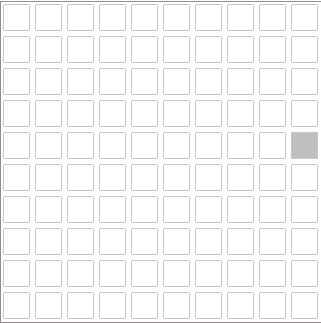
\includegraphics[scale=1]{img/carte.png}
						\captionof{figure}{Image de la carte générée}
   	 				\end{center}


   	 		\subsubsection{Les attributs}
   	 			\paragraph{Listes des attribut}
					\begin{lstlisting}[caption={Attributs classe Carte}]
						// On genere les items sur la carte 
						item = new Item(); 
						// On recupere la carte 
						carte = document.getElementById("carte"); 
						// Nombre de lignes
						x = 10; 
						// Nombre de colonnes
						y = 10; 
						// Tableau des ids des cases selectionnees
						ids = []; 
					\end{lstlisting}
				\paragraph{Description des attributs}
					\begin{itemize}
						\item item = Objet de la classe Item permettant l'instanciation des items
						\item carte = élément du document qui va intégré la carte
						\item x et y = nombre de lignes et de colonnes permettant la définition de la carte
						\item ids = tableaux des identifiants des cases sélectionnées 
					\end{itemize}
				\newpage
   	 		\subsubsection{Les méthodes}
				\paragraph{Listes des méthodes}
					\begin{lstlisting}[caption={Méthodes classe Carte}]
						    // Genere la carte 
						    initCarte(x, y, carte) {}
						    // Regenere la carte si necessaire
		        			regenCarte(x, y, carte) {}
	        				// Gere les clicks
	     				    eventHandler(carte) {}
    						// Gere les clicks sur les noeuds
						    getNodeClicked(event) {}
						    // ajoute les anciens ids des cases cocher dans le tableau "id"
					        ajoutAncienID(id) {}
					        // Affiche tout les ids stockes
					        getAllID()
					        // Renvoie l'ID de l'index choisi
					        getID(index)
   							// Genere les items sur la carte 
   							genItem()
					\end{lstlisting}
				\paragraph{Description des fonctions}
					\begin{itemize}
						\item \textcolor{DarkOrchid}{initCarte(x, y, carte)} = initialise la carte ainsi que les cases clickable,en fonction d'un taille x et y et d'un emplacement de carte
						\item \textcolor{DarkOrchid}{regenCarte(x, y, carte)} = réinitialise la carte avec les mêmes paramètres que initcarte
						\item \textcolor{DarkOrchid}{eventHandler(carte)} = gère les événements de la carte (les clicks), retourne vrai si l'élément cliqué correspond à une case faux sinon
						\item \textcolor{DarkOrchid}{getNodeClicked(event)} = gère quels noeuds ont été cliqués en fonction d'un événement (définit dans eventHandler)
						\item \textcolor{DarkOrchid}{ajoutAncienID(id)} = ajoute l'id cliqué dans le tableau des ids
						\item \textcolor{DarkOrchid}{getAllID()} = affiche tout les items déjà cliqués
						\item \textcolor{DarkOrchid}{getID(index)} = retourne l'id de l'index voulu
						\item \textcolor{DarkOrchid}{genItem()} = génère les items dans la carte, il peut s'agir de malus ou de bonus, fonction pas implémenté à l'heure actuelle.
					\end{itemize}
				\newpage
   	 	\subsection{Classe \textcolor{red}{Message}}
			\subsubsection{Description de la classe}
				\paragraph{But de la classe : }
  	 				La classe \textbf{\textcolor{ForestGreen}{Message}} gère l'affichage des messages dans le jeu. Cette classe ne gère que l'ajout des messages au cours du jeu. 
  	 				Cependant le jeu n'étant pas fini, les messages ne sont pas implémentés.
   	 		\subsubsection{Les attributs}
					\paragraph{Listes des attribut}
					\begin{lstlisting}[caption={Attributs classe Message}]
						// On recupere l'emplacement des messages 
						message = document.getElementById("message");
					\end{lstlisting}
					\paragraph{Description des attributs}
					\begin{itemize}
						\item message = élément du document qui va intégré les messages
					\end{itemize}
   	 		\subsubsection{Les méthodes}
				\paragraph{Listes des méthodes}
				\begin{lstlisting}[caption={Méthodes classe Message}]
					// Genere la zone des messages
				    initMessage() {}
					// Ajoute le contenu du message
					ajoutMessage(contenu)
				\end{lstlisting}
				\paragraph{Description des fonctions}
				\begin{itemize}
					\item \textcolor{DarkOrchid}{initMessage()} = initialise la zone des messages
					\item \textcolor{DarkOrchid}{ajoutMessage(contenu)} = ajoute le message à la zone de message
				\end{itemize}
			\newpage
			
   	 	\subsection{Classe \textcolor{red}{Item}}
			\subsubsection{Description de la classe}
			\paragraph{But de la classe : }
			La classe \textbf{\textcolor{ForestGreen}{Jeu}} gère les items dans le jeu, c'est la classe mère des classes Objet et Malus. 
			Cependant le jeu n'étant pas fini, les Items ne sont pas implémentés.
			\subsubsection{Les attributs}
			\paragraph{Listes des attribut}
			\begin{lstlisting}[caption={Attributs classe Message}]
				// On recupere l'emplacement des messages 
				Zmessage = document.getElementById("message");
				// infos des items
				info = [];
				// Enumeration des effets possibles
				effet = { MALUS: 1, BONUS: 0 };

			\end{lstlisting}
			\paragraph{Description des attributs}
			\begin{itemize}
				\item Zmessage = élément du document qui va intégré les messages
				\item info = tableaux contenant les informations des items
				\item effet = énumérations des possibilités qu'il s'agissent d'un malus ou d'un bonus
			\end{itemize}
			\subsubsection{Les méthodes}
			\paragraph{Listes des méthodes}
			\begin{lstlisting}[caption={Méthodes classe Message}]
				// Retourne le nom de l'item
				getNom() {}
				// Met le nom d'un item a jour
				setNom(nom)
				// Retourne l'effet de l'item (malus ou bonus)
				getEffet() {}
				// Met a jour effet
				setEffet(effet) {}
				// Prototype de fonction permettant la generation d'un nb aleatoire d'item (utile pour les sous classes)
				nbAleat(value) {}
				// Ajoute l'item dans la liste info
				ajoutItem(obj)
				// Retourne le nombre d'item present la liste info
				getNbItem()
				// Renvoie les infos d'un objet
				getInfosObjets()
				// ajout d'un message dans la zone de message
				addMessage(obj)
			\end{lstlisting}
			\paragraph{Description des fonctions}
			\begin{itemize}
				\item \textcolor{DarkOrchid}{getNom(), setNom()} = getter / setter du nom de l'objet
				\item \textcolor{DarkOrchid}{getEffet(), setEffet()} = getter / setter de l'effet objet
				\item \textcolor{DarkOrchid}{ajoutMessage(contenu)} = ajoute le message à la zone de message
				\item \textcolor{DarkOrchid}{nbAleat(value)} = génère un nombre d'item aléatoire entre 1 et value 
				\item \textcolor{DarkOrchid}{ajoutItem(obj)} = ajoute l'item dans la liste info
				\item \textcolor{DarkOrchid}{getNbItem()} = renvoie le nombre d'item présent dans la liste info
				\item \textcolor{DarkOrchid}{getInfosObjets()} = renvoie les infos d'un item dans la liste info
				\item \textcolor{DarkOrchid}{addMessage(obj)} = ajoute un message dans la zone de message
			\end{itemize}
\end{document}